\newpage
\section{Aufgabenstellung}

Das Ziel der \acrfull{pren1} und 2 ist das Planen und Verwirklichen eines vollkommen autonomen Roboters. Die Anforderungen an diesen Roboter werden anschliessend vereinfacht behandelt. 
 
\begin{figure}[H]
  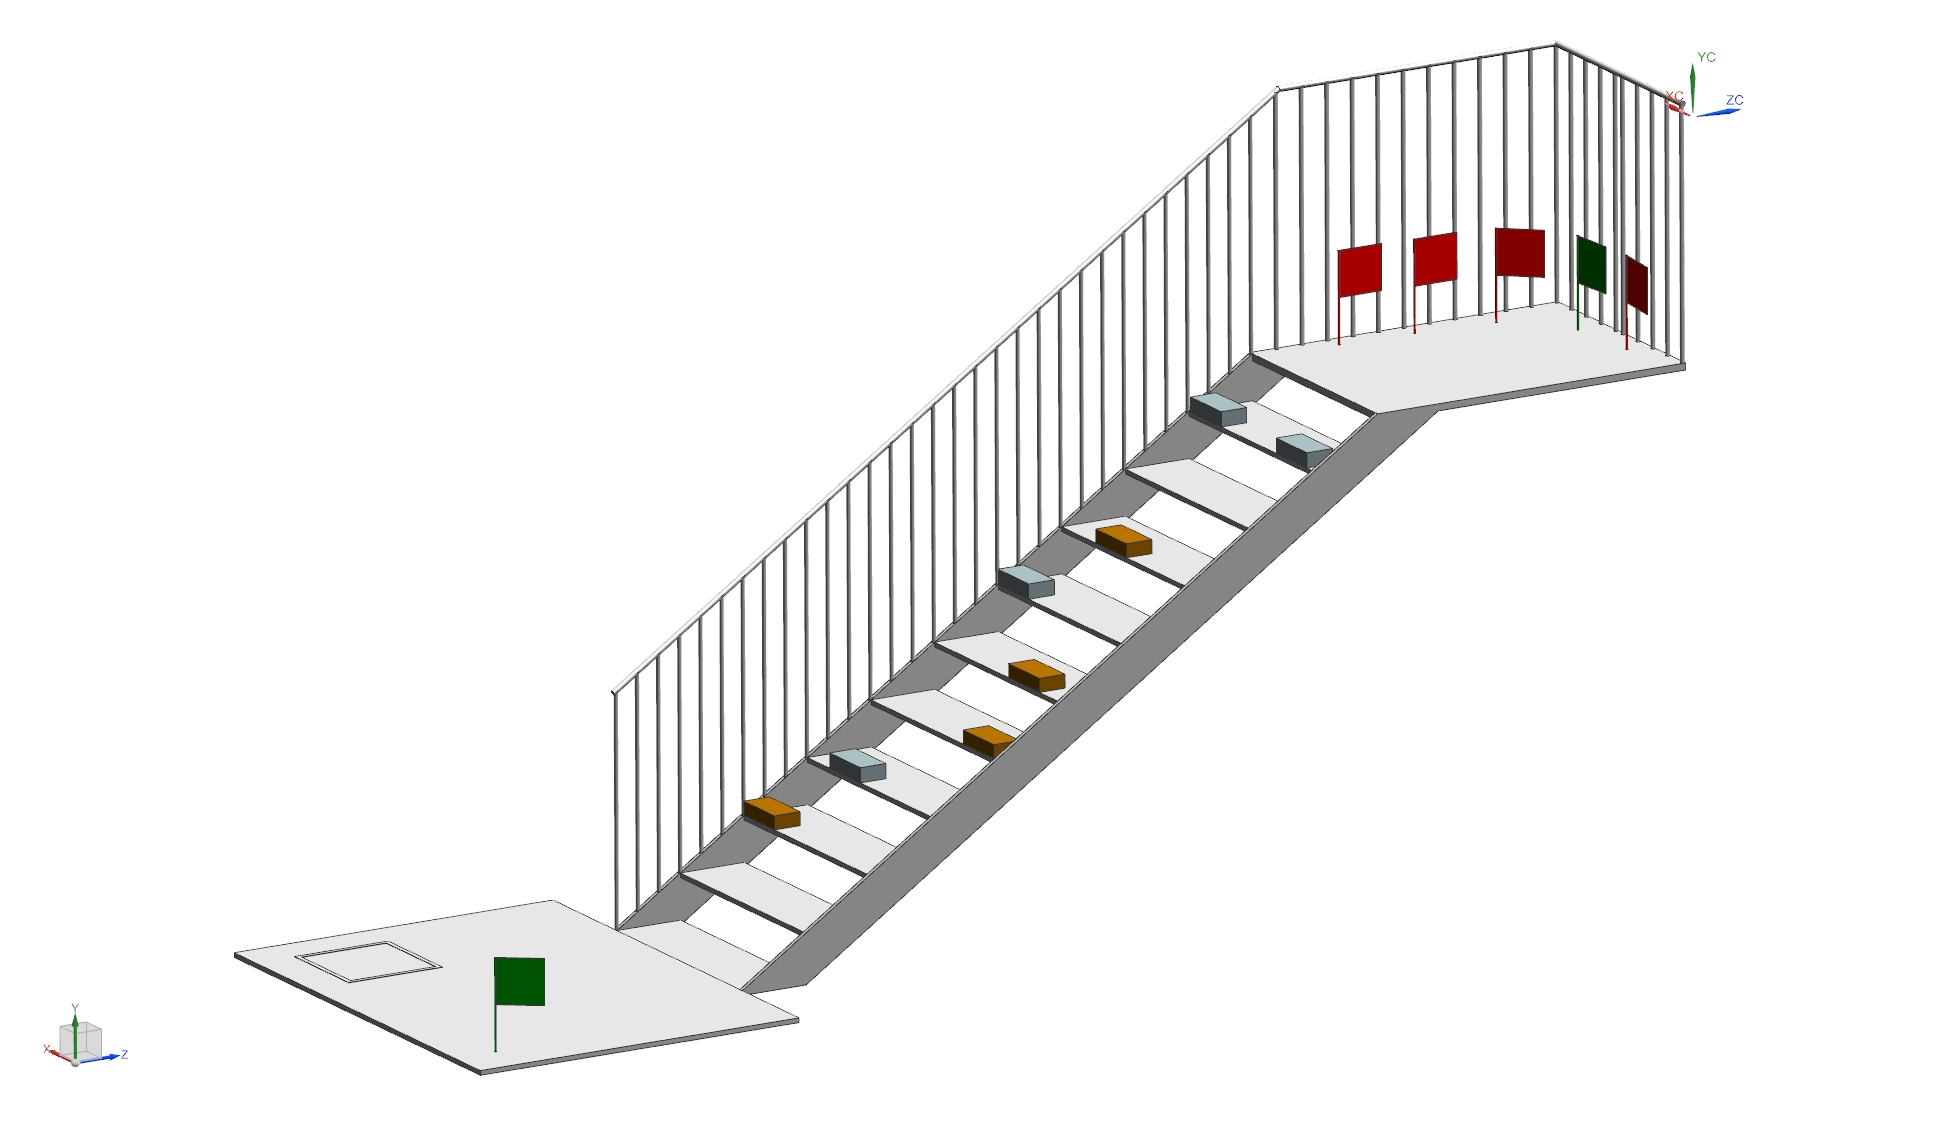
\includegraphics[width=1\textwidth]{img/Aufgabenstellung.png}
  \centering
  \caption{Skizzierung der Treppe}
  \label{fig:seitenansicht-treppe}
\end{figure}
 
Das Team hat zwei Minuten, um den Roboter auf dem Spielfeld in dem 40x40 cm grossen 
Startfeld (siehe Abbildung \ref{fig:seitenansicht-treppe}) zu positionieren und letzte Vorkehrungen zu treffen. Danach wird der Roboter mittels eines einzelnen Tasters gestartet. 
Für alle folgenden Aufgaben hat er maximal vier Minuten zur Verfügung. 
Die autonome Maschine sucht zuerst im Startbereich ein Piktogramm, welches zufällig aus fünf möglichen Piktogrammen ausgewählt wird.

\newpage

Hat der Roboter dieses Bild gefunden, bestätigt er dies dem Publikum. Nun muss die Treppe bestiegen werden. Um die Aufgabe zusätzlich zu erschweren, werden auf der Treppe zufällig zwei verschiedene Ziegelsteinarten positioniert, welche der Roboter selbständig um- oder überfahren soll, ohne diese zu verschieben. Dies wird in der Abbildung \ref{fig:treppe-aufriss-boden} dargestellt. Ist die obere Plattform erreicht, steht der Roboter vor dem letzten Teil der Aufgabe. Aus allen fünf verfügbaren, aufgestellten Piktogrammen muss die Kopie jenes aus dem Startbereich gefunden werden. Wurde das richtige Piktogramm identifiziert, muss dies wiederum signalisiert werden. Das Team darf, wenn der Roboter einmal gestartet ist, keinen Einfluss mehr auf das Geschehen nehmen und hat maximal zwei solcher Durchläufe,
um die Aufgabe zu bewältigen. Für diese Aufgaben darf die Maschine nicht mehr als 100 cm vom Boden abheben oder das Geländer zur Hilfe nehmen. Eine Fortbewegung mittels Ketten- oder Raupenantriebes ist ebenfalls nicht erlaubt.

Nachfolgend ist die Treppe von der Startfläche aus verschiedenen Höhen zu sehen, um einen Eindruck zu verleihen, wie der Roboter die Aufgabenstellung sieht. Abbildung \ref{fig:treppe-aufriss-boden} zeigt die Treppe mit Sicht vom Boden aus, die Abbildung \ref{fig:treppe-aufriss-0.5m} zeigt die Treppe aus der Sicht von 0.5 m Höhe und die Abbildung \ref{fig:treppe-aufriss-1m} aus 1 m Höhe.

\begin{figure}[H]
  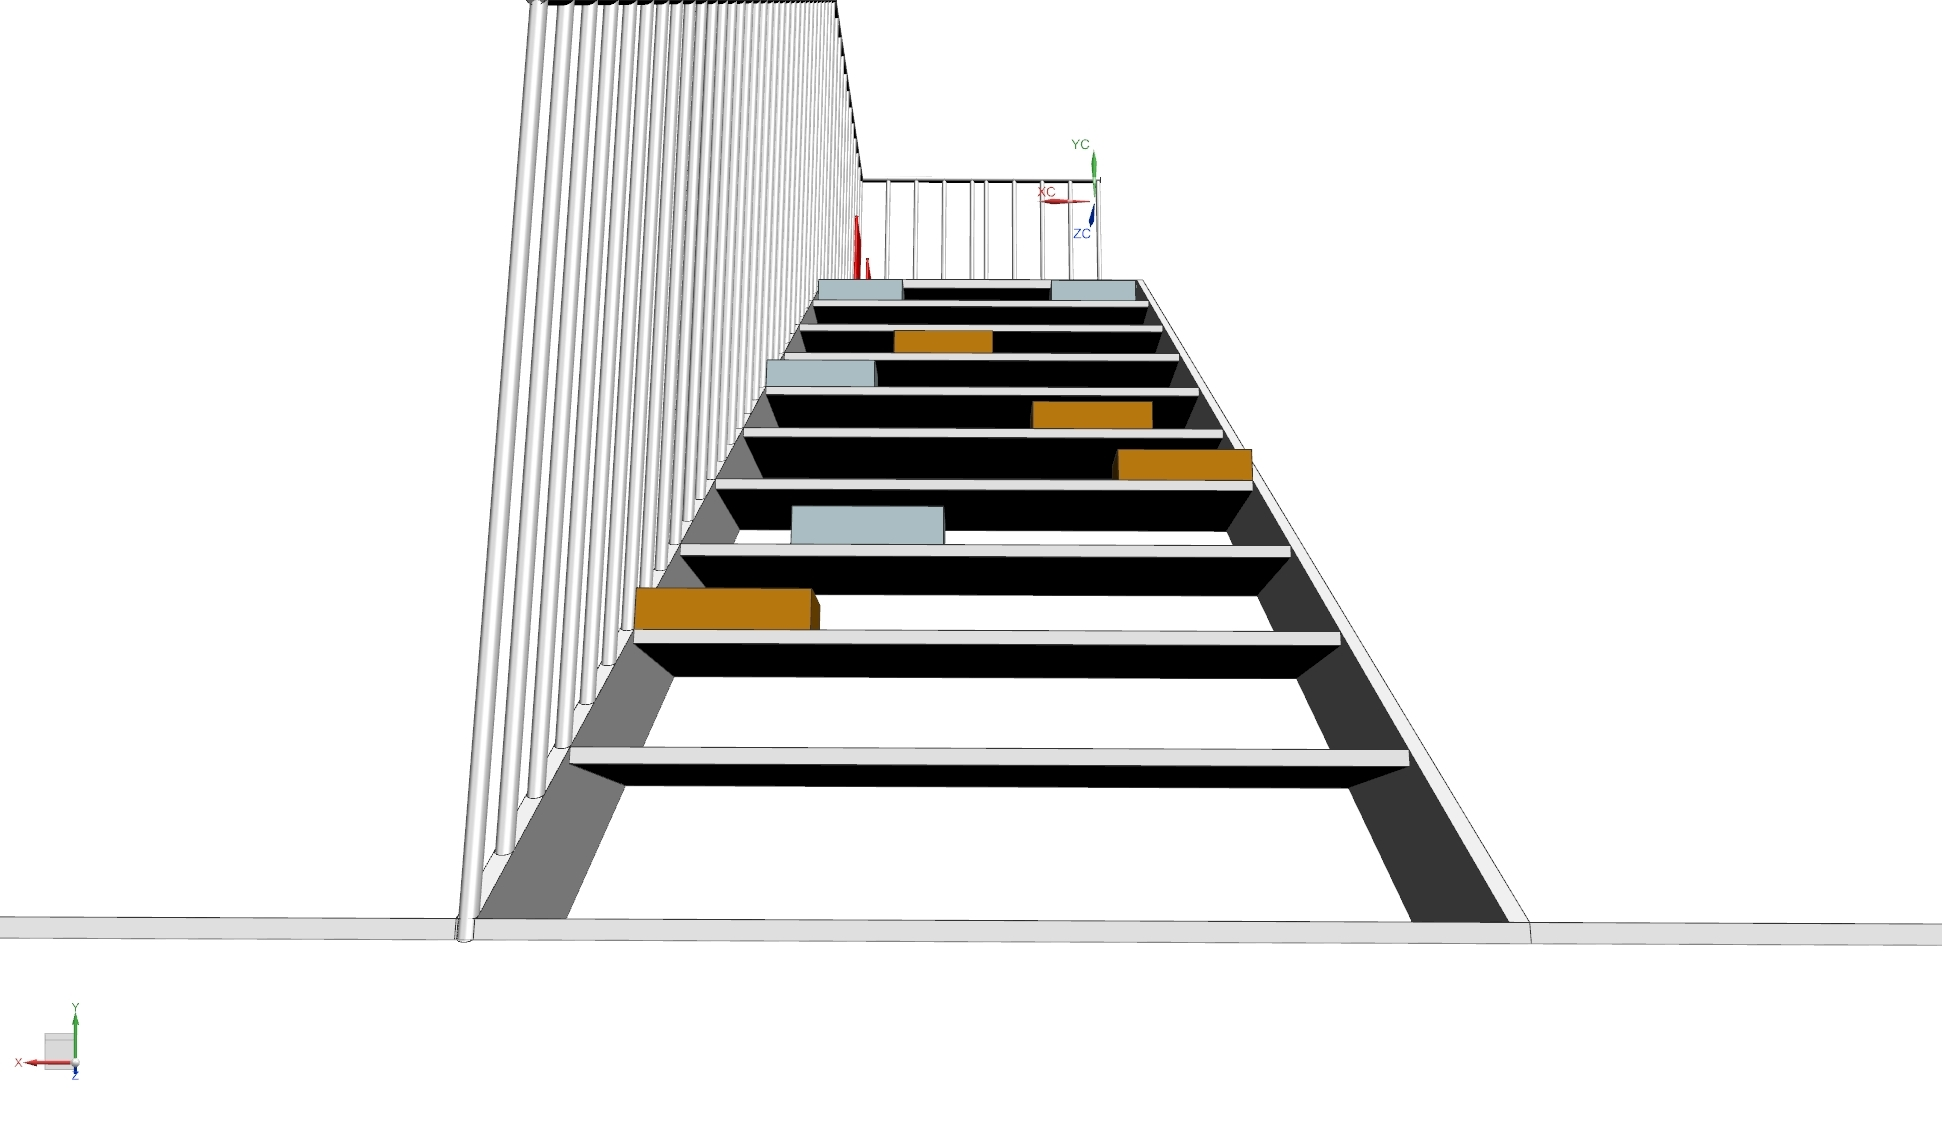
\includegraphics[width=1\textwidth]{img/Boden.png}
  \centering
  \caption{Die Treppe vom Boden des Startbereiches aus}
  \label{fig:treppe-aufriss-boden}
\end{figure}

\newpage

\begin{figure}[H]
  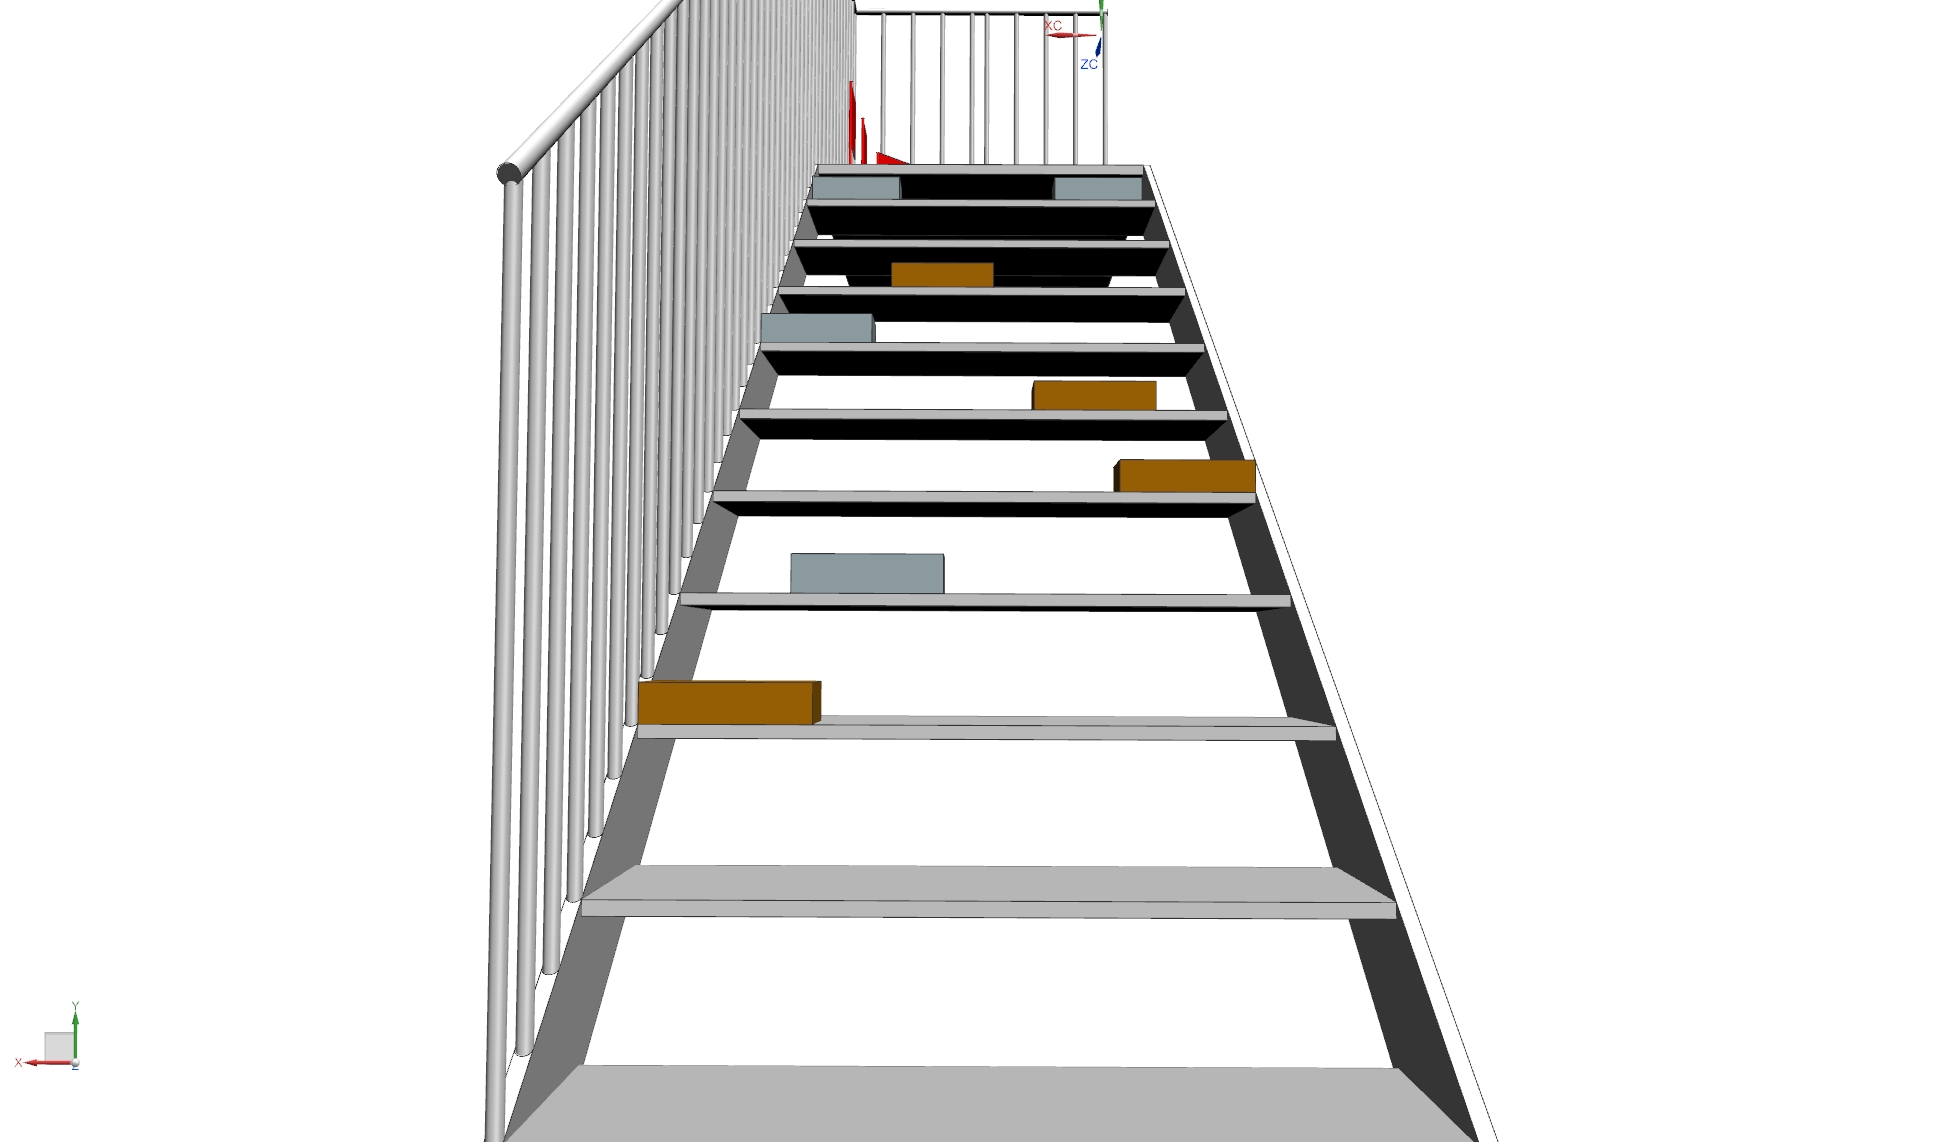
\includegraphics[width=1\textwidth]{img/500mm.png}
  \centering
  \caption{Die Treppe mit dem Betrachter auf 0.5 m Höhe}
  \label{fig:treppe-aufriss-0.5m}
\end{figure}

\begin{figure}[H]
  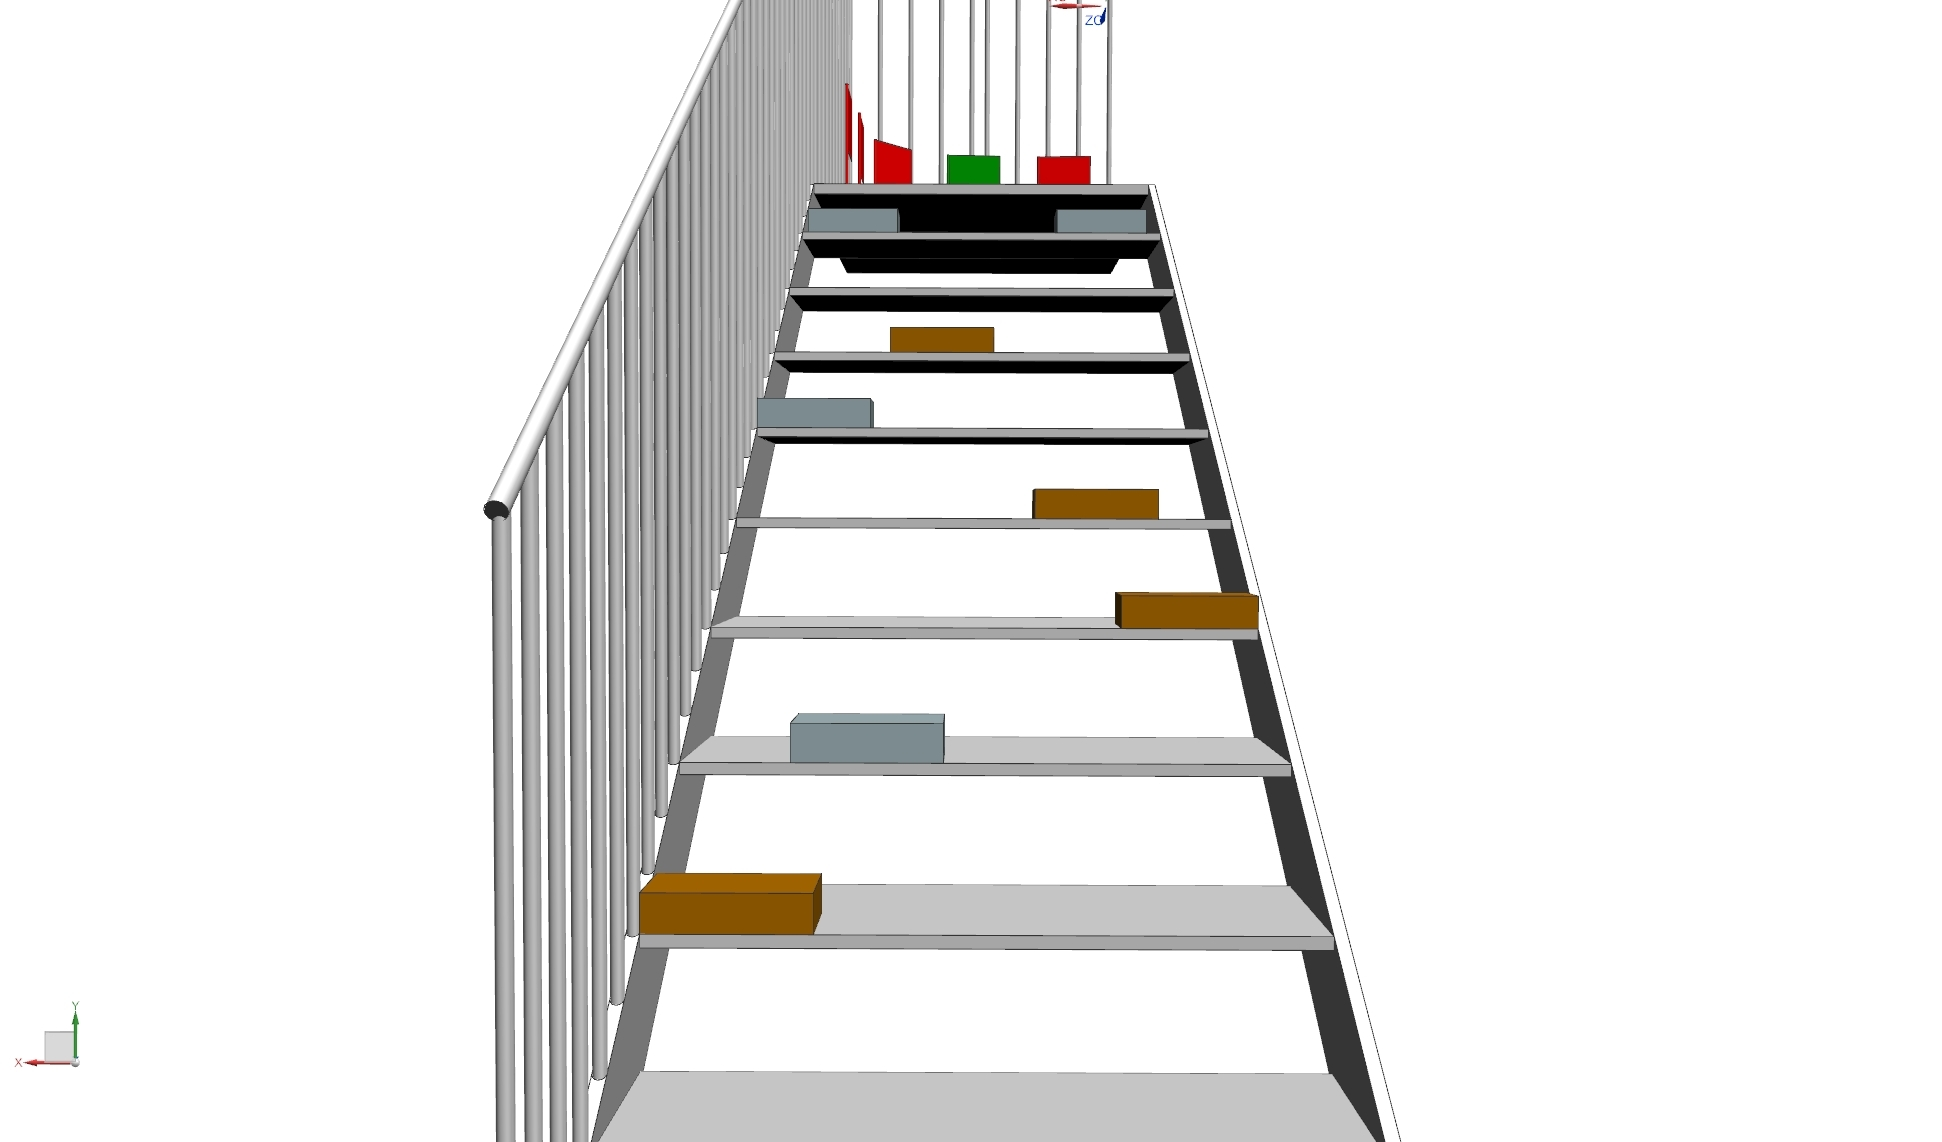
\includegraphics[width=1\textwidth]{img/1000mm.png}
  \centering
  \caption{Die Treppe mit dem Betrachter auf 1 m Höhe}
  \label{fig:treppe-aufriss-1m}
\end{figure}

